\documentclass[11pt]{article}
\usepackage[margin=1in]{geometry}
\usepackage{amsmath,amssymb,amsfonts,bm,mathtools}
\usepackage{tikz}
\usetikzlibrary{arrows.meta,positioning,shapes.geometric}
\usepackage{hyperref}

\title{Euclidean VAE: Rigorous Mathematical Formulation}
\date{}

\begin{document}
\maketitle

\section{Setup}
Let $x\in\mathbb{R}^p$ be a preprocessed input vector and $z\in\mathbb{R}^d$ a latent variable.
The prior is
\begin{equation}
p(z)=\mathcal N(0,I_d).
\end{equation}
The encoder defines a diagonal Gaussian posterior
\begin{equation}
q_\phi(z\mid x)=\mathcal N\big(\mu_\phi(x),\operatorname{diag}(\sigma_\phi^2(x))\big).
\end{equation}

\section{Encoder and decoder}
With MLP hidden states $h^{(\ell)}$:
\begin{equation}
h^{(\ell)}=\sigma\!\big(W^{(\ell)}h^{(\ell-1)}+b^{(\ell)}\big),
\qquad h^{(0)}=x.
\end{equation}
Posterior parameters are
\begin{equation}
\mu = W_\mu h^{(L)} + b_\mu,
\qquad
\log\sigma^2 = W_{\log\sigma^2} h^{(L)} + b_{\log\sigma^2}.
\end{equation}
Reparameterization:
\begin{equation}
z=\mu+\sigma\odot\varepsilon,
\qquad
\sigma=\exp\!\left(\tfrac12\log\sigma^2\right),
\qquad
\varepsilon\sim\mathcal N(0,I_d).
\end{equation}
Decoder output:
\begin{equation}
\hat x=f_\theta(z).
\end{equation}

\section{KL divergence}
For diagonal Gaussian posterior and standard normal prior,
\begin{equation}
\mathrm{KL}\big(q_\phi(z\mid x)\|p(z)\big)
=\frac12\sum_{j=1}^d\left(\mu_j^2+\sigma_j^2-1-\log\sigma_j^2\right)
= -\frac12\sum_{j=1}^d\left(1+\log\sigma_j^2-\mu_j^2-e^{\log\sigma_j^2}\right).
\end{equation}

\section{Reconstruction penalties}
\paragraph{MSE}
\begin{equation}
\mathcal L_{\mathrm{rec}}^{\mathrm{MSE}}=\frac1p\sum_{i=1}^p(\hat x_i-x_i)^2.
\end{equation}
\paragraph{MAE}
\begin{equation}
\mathcal L_{\mathrm{rec}}^{\mathrm{MAE}}=\frac1p\sum_{i=1}^p|\hat x_i-x_i|.
\end{equation}
\paragraph{Huber ($\delta>0$)}
\begin{equation}
\mathcal L_{\mathrm{rec}}^{\mathrm{Huber}}
=\frac1p\sum_{i=1}^p
\begin{cases}
\tfrac12(\hat x_i-x_i)^2,& |\hat x_i-x_i|\le\delta,\\
\delta\left(|\hat x_i-x_i|-\tfrac12\delta\right),& \text{otherwise}.
\end{cases}
\end{equation}

\section{Training objectives}
\subsection*{$\beta$-VAE}
\begin{equation}
\mathcal J_\beta(x)
=\mathcal L_{\mathrm{rec}}(x,\hat x)
+\beta_t\,\mathrm{KL}\big(q_\phi(z\mid x)\|p(z)\big),
\end{equation}
with warmup schedule
\begin{equation}
\beta_t=\min\!\left(\beta_{\max},\beta_{\max}\frac{t}{T_{\mathrm{warmup}}}\right).
\end{equation}

\subsection*{Capacity objective}
\begin{equation}
\mathcal J_{\mathrm{cap}}(x)
=\mathcal L_{\mathrm{rec}}(x,\hat x)
+\gamma\,\left|\mathrm{KL}(q_\phi\|p)-C_t\right|.
\end{equation}

\subsection*{Free bits}
\begin{equation}
\mathrm{KL}_{\mathrm{fb}}=\sum_{j=1}^d\max\{\mathrm{KL}_j,\lambda_{\mathrm{fb}}\}.
\end{equation}

\section{ELBO interpretation}
The negative ELBO is
\begin{equation}
-\mathcal L_{\mathrm{ELBO}}
=-\mathbb E_{q_\phi(z\mid x)}[\log p_\theta(x\mid z)]
+\mathrm{KL}(q_\phi\|p).
\end{equation}
In practice, MSE/MAE/Huber provide surrogate reconstructions while preserving exact KL regularization.

\section{Diagram}
\begin{center}
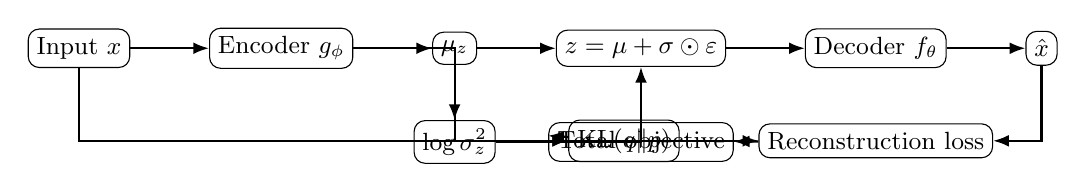
\begin{tikzpicture}[
  node distance=7mm and 10mm,
  box/.style={draw,rounded corners,align=center,inner sep=3pt,font=\small},
  arr/.style={-{Latex[length=2mm]},thick}
]
\node[box] (x) {Input $x$};
\node[box, right=of x] (enc) {Encoder $g_\phi$};
\node[box, right=of enc] (mu) {$\mu_z$};
\node[box, below=of mu] (lv) {$\log\sigma_z^2$};
\node[box, right=of mu] (z) {$z=\mu+\sigma\odot\varepsilon$};
\node[box, right=of z] (dec) {Decoder $f_\theta$};
\node[box, right=of dec] (xh) {$\hat x$};
\node[box, below=of dec] (rec) {Reconstruction loss};
\node[box, left=of rec] (kl) {KL$(q\|p)$};
\node[box, below=of z] (loss) {Total objective};

\draw[arr] (x) -- (enc);
\draw[arr] (enc) -- (mu);
\draw[arr] (enc) -| (lv);
\draw[arr] (mu) -- (z);
\draw[arr] (lv) -| (z);
\draw[arr] (z) -- (dec);
\draw[arr] (dec) -- (xh);
\draw[arr] (xh) |- (rec);
\draw[arr] (x) |- (rec);
\draw[arr] (mu) |- (kl);
\draw[arr] (lv) |- (kl);
\draw[arr] (rec) -- (loss);
\draw[arr] (kl) -- (loss);
\end{tikzpicture}
\end{center}

\end{document}
